% !TeX root = ../main.tex

\chapter{Background}\label{chapter:background}

\section{Visual Odometry Foundations}

Visual odometry estimates a time-ordered sequence of camera poses from visual observations. A visual frontend supplies correspondences between frames, while a backend uses their geometric constraints to estimate motion. Visual SLAM extends this local estimation problem with a persistent map and mechanisms for global consistency, such as loop closure~\cite{cadena2016past}. This thesis evaluates local trajectory estimation and therefore uses the term visual odometry unless a cited system explicitly provides broader SLAM functionality.

Let $\mathcal{F}_W$ denote the world frame and $\mathcal{F}_{C_t}$ the camera frame at time $t$. The pose $\mathbf{T}_{WC_t}\in\mathrm{SE}(3)$ maps a point from $\mathcal{F}_{C_t}$ to $\mathcal{F}_W$ and contains a rotation $\mathbf{R}_{WC_t}\in\mathrm{SO}(3)$ and translation $\mathbf{t}_{WC_t}\in\mathbb{R}^3$. A landmark $\mathbf{p}_j^W$ is a scene point expressed in the world frame. Two-dimensional observations assigned to the same landmark form a track. Frames retained for joint pose and landmark refinement are called keyframes; limiting their number bounds the optimization problem.

\section{Camera and Stereo Geometry}

A calibrated central camera is described by a projection $\pi:\mathbb{R}^3\rightarrow\mathbb{R}^2$ and an inverse projection $\pi^{-1}$ that maps an image coordinate to a viewing ray. For the pinhole model,
\begin{equation}
  \pi\!\left(\begin{bmatrix}X&Y&Z\end{bmatrix}^{\mathsf T}\right)
  = \begin{bmatrix}f_x X/Z+c_x & f_y Y/Z+c_y\end{bmatrix}^{\mathsf T}.
\end{equation}
Native projections may additionally include lens distortion; rectification instead remaps both stereo cameras to a shared virtual, undistorted projection~\cite{hartley2004multiple}.

The calibrated stereo extrinsics fix the relative rotation and translation between the anchor and stereo views, and the translation magnitude defines the baseline. A point observed in one view must lie on the corresponding epipolar line in the other. Rectification makes these lines horizontal, so correspondence reduces to a one-dimensional disparity search. In the ideal parallel pinhole case, depth is $Z=f b/d$ for focal length $f$, baseline $b$, and disparity $d$. More generally, depth is obtained by triangulating the two calibrated rays. A valid reconstruction must satisfy cheirality, placing the point in front of both cameras~\cite{hartley2004multiple}.

\section{Nonlinear Optimization for Visual Odometry}

For an observation $\mathbf{u}_{j,t}$ of landmark $j$ at time $t$, the conventional reprojection residual uses the predicted-minus-measured convention,
\begin{equation}
  \mathbf{e}_{j,t}
  = \pi\!\left(\mathbf{T}_{WC_t}^{-1}\mathbf{p}_j^W\right)
  - \mathbf{u}_{j,t}.
\end{equation}
Bundle adjustment is the joint refinement of scene structure and viewing parameters by minimizing a cost over their prediction errors~\cite{triggs2000bundle}. For point-based visual odometry, each landmark couples the poses from which it is observed. A longer, correctly associated track can therefore support the same structure from several views, while a two-frame track supplies only a pairwise constraint. This additional support is useful only when the observations are geometrically consistent; an incorrect long association can instead contaminate several states. A robust loss, such as the Huber loss, reduces the influence of observations whose residuals are inconsistent with the assumed noise model~\cite{huber1964robust}.

The visual-only Basalt backend used here retains the bounded-window formulation of its visual-inertial estimator~\cite{usenko2020visual}. Recent states and selected keyframes remain active in the optimization; variables leaving the window are marginalized and their information is retained as a prior. This standard marginalization remains enabled in the frozen configuration, whereas the separately evaluated pre-marginalization outlier filter and second optimization pass are not retained. Since visual measurements constrain only relative geometry, a reference pose must be fixed to remove the global gauge freedom. The proposed residual changes the visual measurement term but retains this state-management structure; it is defined in \autoref{chapter:method}.

\section{H.264 Inter Prediction and Motion Vectors}

\subsection{Prediction, Residuals, and Reconstruction}

H.264, also called Advanced Video Coding (AVC) or MPEG-4 Part 10, represents
video through a standardized compressed syntax and decoding
process~\cite{Wiegand2003Overview,ITUT_H264_2026}. H.264 uses a block-based
hybrid coding model combining inter-picture prediction with transform coding
of the prediction residual~\cite[Sec.~IV]{Wiegand2003Overview}.
The following explanation concerns the progressive-frame, 4:2:0 setting used
in this thesis; interlaced and multiview extensions are not required.

Prediction reduces the amount of new information needed to describe a block.
Intra prediction uses already reconstructed neighbouring samples within the
current picture. Inter prediction instead uses a displaced region of a
reference picture. A motion vector describes the displacement used for motion
compensation~\cite[Sec.~3.95]{ITUT_H264_2026}. In addition to prediction information,
the encoder can transmit a residual: the difference between the input block and
its prediction. This residual is transformed, quantized, and entropy coded.
The decoder reconstructs the residual and adds it to the prediction; an in-loop
deblocking filter can then modify the reconstructed samples. Reference pictures
are reconstructed pictures, so encoder and decoder use matching reference
content rather than the encoder's uncompressed input
images~\cite[Sec.~IV]{Wiegand2003Overview}.

Motion vectors alone therefore do not determine the decoded image. Prediction
can be imperfect while the coded residual restores image detail. The
quantization parameter controls residual-coefficient quantization, not the
spatial step of the motion-vector representation. A visually acceptable decoded
frame need not have geometrically accurate motion
vectors~\cite{Wiegand2003Overview,young2020fast}.

Crucially, the standard specifies which bitstreams are valid and how they are
decoded, not a unique motion-estimation algorithm
\cite[Sec.~3.52]{ITUT_H264_2026}. Motion search, partition selection, and rate
control are encoder decisions. Their purpose is compression efficiency, often
expressed by a rate-distortion objective of the form
\begin{equation}
  J(c)=D(c)+\lambda R(c),
  \label{eq:codec-rate-distortion}
\end{equation}
where $c$ is a coding choice, $D$ measures reconstruction distortion, $R$ counts
its required bits, and $\lambda$ trades distortion against rate. Choices include
the prediction mode, partitioning, reference picture, motion vectors, and
residual coding. Practical searches can use approximations and early exits;
H.264 compliance does not imply a globally optimal search or identical vectors
from different encoders~\cite{Wiegand2003Overview}. The rate cost makes a vector
that is cheap to describe competitive with one that better matches image
appearance, even before geometric interpretation is considered.

\subsection{Spatial Support and Partitioning}

In 4:2:0 video, the luma component represents brightness, while each chroma
component is sampled at half the horizontal and vertical luma resolution.
The spatial dimensions used below are in luma samples. A macroblock covers
$16\times16$ luma samples. Inter prediction can use that region as one block or
partition it into $16\times8$, $8\times16$, or $8\times8$ regions. Each
$8\times8$ region can independently remain whole or be subdivided into
$8\times4$, $4\times8$, or $4\times4$ subpartitions
\cite[Tables~7-13 and~7-17]{ITUT_H264_2026}. The hierarchy is illustrated in
\autoref{fig:h264-prediction-partitions}. H.264 therefore does not require a
uniform grid of $8\times8$ motion vectors.

\begin{figure}[htbp]
  \centering
  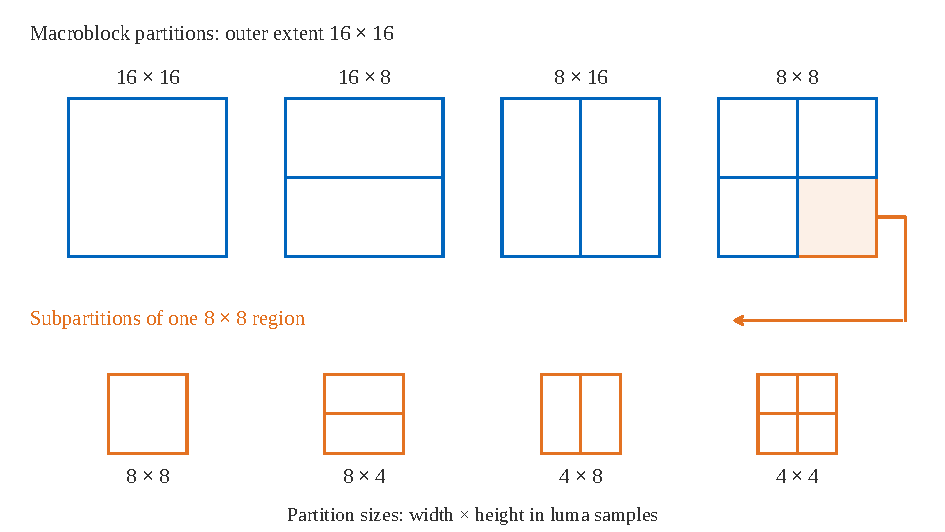
\includegraphics[width=\textwidth]{figures/background/h264-prediction-partitions}
  \caption[H.264 inter-prediction partitions]{H.264 inter-prediction partition choices in luma samples. Top:
  partitioning of a $16\times16$ macroblock. Bottom: possible subdivisions of
  one $8\times8$ region; the four regions of a partitioned macroblock can
  select these independently. The drawing uses a common spatial scale and
  shows prediction support, not transform blocks. Based on
  \cite[Tables~7-13 and~7-17]{ITUT_H264_2026}.}
  \label{fig:h264-prediction-partitions}
\end{figure}

Each inter-predicted partition or subpartition carries a translational motion
description, with one vector for a unidirectionally predicted block. Larger
partitions reduce the motion information to encode; smaller ones can represent
different displacements within the same macroblock at greater signalling cost.
These regions are not feature detections or object segments. Their selection
can change between pictures without preserving any identity
\cite[Sec.~IV-H]{Wiegand2003Overview}.

Prediction support must also be distinguished from residual transform size.
For example, the $4\times4$ transform operates on prediction-error samples; it
does not imply that every inter-prediction vector belongs to a $4\times4$
region. High-profile coding additionally permits an $8\times8$ transform
\cite[Secs.~8.5 and~A.2.4]{ITUT_H264_2026}. The MV block dimensions describe
where a displacement is applied, not the precision with which a point inside
that region has been localized.

\subsection{Reference Pictures and Temporal Direction}

Pictures are divided into slices, whose types constrain the available coding
modes. An I slice uses intra coding. A P slice permits intra coding and
inter prediction from one reference list; a B slice additionally permits a
prediction combining two reference lists. P and B slices can therefore contain
intra-coded regions with no inter-picture motion vector
\cite[Table~7-10]{ITUT_H264_2026}. The common terms I-, P-, and B-frame are
shorthand; a P label alone does not imply a temporal vector at every location.
An instantaneous decoding refresh (IDR) picture also resets reference-picture
dependencies. An ordinary intra-coded picture does not necessarily prevent
later pictures from referring to pictures preceding it
\cite[Sec.~3.69]{ITUT_H264_2026}.
A pattern such as I-P-P specifies coding types, but does not by itself specify
every reference relationship~\cite[Secs.~7.4.5 and~8.2.4]{ITUT_H264_2026}.

A vector is meaningful only together with its reference-picture identity.
H.264 can retain multiple reconstructed references, and decoding order need
not equal display order. In B prediction, either reference list can contain
pictures from either temporal direction; a list index is not by itself a
timestamp or a direction of motion
\cite[Secs.~IV-H.1 and~IV-H.2]{Wiegand2003Overview}.

The direction convention matters. Under a current-to-reference lookup
convention, a vector $\mathbf{m}$ pairs a location $\mathbf{q}$ in the current
coding block with $\mathbf{q}+\mathbf{m}$ in the reference
image~\cite[Sec.~3.95]{ITUT_H264_2026}. If the reference
is the preceding frame, forward-time propagation instead maps a point
$\mathbf{p}$ in that reference support to $\mathbf{p}-\mathbf{m}$. Thus an encoder
reference arrow and a forward-time motion arrow have opposite directions in
this case. For example, a horizontal lookup displacement of $-2$ pixels describes
a forward-time displacement of $+2$ pixels between those supports. It is a
displacement over the reference interval, not a velocity.

The experiments restrict reference count and prediction structure to simplify
this interpretation (\autoref{chapter:experimental-methodology}). Encoding the
same images in reverse order is nevertheless a new prediction problem, not a
way to obtain the exact inverse of the original vectors. This independently
encoded reverse stream is also distinct from the two reference lists of a
single B slice. Neither codec syntax nor rate-distortion optimization enforces
reciprocal agreement between the two encodings.

\subsection{Subpixel Precision and Decoded Motion Information}

H.264 represents luma motion in quarter-sample units. An integer vector
component $k$ therefore represents $k/4$ luma pixels, allowing displacements
between recorded sample locations. Motion compensation obtains these
fractional reference samples by interpolation: half-sample luma positions use
a six-tap filter, and quarter-sample positions use rounded averages of suitable
integer- and half-sample values
\cite[Secs.~8.4.2.2 and~8.4.2.2.1]{ITUT_H264_2026}. In 4:2:0 chroma, the
same displacement corresponds to eighth-chroma-sample units because that grid
has half the luma resolution; this does not provide eighth-pixel precision on
the luma image~\cite[Sec.~8.4.1.4]{ITUT_H264_2026}.

Fractional precision specifies representable displacements, not a bound on
error relative to physical image motion. The chosen vector is the result of
prediction search and coding decisions, not necessarily a correctly estimated
continuous motion rounded to its nearest quarter pixel. Consequently,
$0.25$-pixel representation alone justifies neither subpixel correspondence
accuracy nor a particular statistical uncertainty model.

The bitstream usually codes a motion-vector difference relative to a predicted
vector. For each component, reconstruction has the form
\begin{equation}
  \mathbf{m}=\mathbf{m}_{\mathrm{pred}}+\Delta\mathbf{m},
\end{equation}
where the predictor depends on neighbouring motion information, partition
shape, and reference indices
\cite[Sec.~8.4.1, Eqs.~(8-172) and~(8-173)]{ITUT_H264_2026}. A zero coded
difference is therefore not necessarily a zero displacement. The codec's
neighbour-based prediction, which includes median-based cases, saves bits;
it is separate from the motion-vector outlier filter introduced in
\autoref{chapter:method}.

Skip and direct modes provide another important distinction. A skipped P
macroblock has inferred motion information despite carrying no explicit
motion-vector difference or residual. Its derived vector need not be zero.
B direct and skip modes likewise derive motion from other decoded information
\cite[Secs.~8.4.1.1 and~8.4.1.2]{ITUT_H264_2026}. This differs from intra
coding, which provides no inter-picture vector. Extracting motion therefore
requires syntax parsing and reconstruction of motion information, including
inferred modes and reference identities, not simply reading explicit vector
differences. The standard separates this derivation from the subsequent use of
reference intensities for motion compensation
\cite[Secs.~8.4.1 and~8.4.2]{ITUT_H264_2026}. The estimator in this thesis
uses the resulting metadata, not the reconstructed intensity samples; this
does not mean that no compressed syntax is decoded.

\subsection{Motion Vectors versus Optical Flow and Feature Tracks}

Optical flow describes apparent image motion between images. A common local
model seeks a displacement $\mathbf{f}$ satisfying brightness constancy,
\begin{equation}
  I_{t+1}(\mathbf{u}+\mathbf{f}(\mathbf{u}))\approx I_t(\mathbf{u}),
\end{equation}
with spatial assumptions or patch support resolving otherwise ambiguous
matches. KLT uses such image information to refine a point displacement;
texture is needed to constrain that displacement in both directions
\cite{shi1994good,young2020fast}. Occlusion, changing illumination, repeated
patterns, and the aperture problem still limit optical-flow estimates: an
isolated straight edge does not constrain displacement along its own direction.
Optical flow is therefore not synonymous with ground-truth scene
correspondence.

Codec motion and optical flow are related because both exploit displaced image
appearance. Their objectives and outputs differ. Codec prediction trades
distortion against coded bits, may use a non-adjacent reference, and assigns one
translation to an entire prediction region. It can leave mismatched appearance
to the coded residual. Optical-flow estimation instead seeks an image-motion
field, without a cost for encoding its vectors in an H.264 stream. Repeating a
block vector at every covered pixel produces a dense array, but adds no
independent motion measurements or localized features. A useful prediction of
the block's appearance can therefore differ from the motion of a particular
corner or edge inside it~\cite{young2020fast,hilscher2026voca}.

\begin{figure}[htbp]
  \centering
  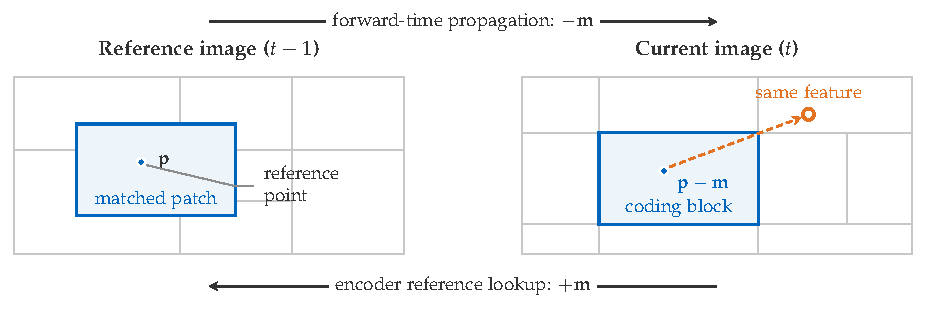
\includegraphics[width=\textwidth]{figures/background/mv-block-prediction}
  \caption[Block prediction and physical feature motion]{Conceptual block prediction, not measured data. Blue rectangles
  mark a matched reference patch and its current coding block. Applying their
  displacement to the reference point produces the filled blue point; the
  same physical feature may appear elsewhere (orange ring). Gray lines show
  independently chosen coding partitions. The arrows distinguish encoder
  reference lookup from chronological propagation for an earlier reference.}
  \label{fig:mv-block-prediction}
\end{figure}

As illustrated in \autoref{fig:mv-block-prediction}, translating a point with
its containing block does not establish feature identity. A matched reference
patch need not coincide with a coding partition in the reference image.
Although coding partitions cover the current picture, their displaced
reference supports can overlap and leave gaps. Repeatedly selecting a block
that covers a propagated point can consequently switch the image structure
being followed. Conversely, a visible structure may have no usable vector:
its region may be intra-coded, or no available source support may cover the
queried point. Missing support supplies no motion measurement and does not
imply that the point is stationary. Measured examples of departure from a KLT
track and abrupt loss of local support are given in
\autoref{fig:mv-feature-departure-example} and
\autoref{fig:mv-abrupt-stop-example}.

Even the presence of a syntactically valid vector does not guarantee a valid
geometric observation. H.264 permits reference lookup outside the image by
extending boundary samples~\cite[Sec.~IV-H.1]{Wiegand2003Overview}; those
extended samples do not constitute additional observed scene content. This
motivates separating codec validity from the image bounds and rectification
validity required for the geometry used here.

\subsection{Texture and the Motion-Matching Error Surface}

The reliability of a block displacement also depends on the shape of its local
matching-error surface. Zhang et al.~\cite{zhang2010subpixel} characterize this
surface from the nine integer-pixel displacements centred on an integer-pixel
optimum. For an image-matching distortion expressed as a sum of squared
differences, the local surface is
\begin{equation}
  E(\Delta x,\Delta y)
  = \sum_{(x,y)\in W}
    \left[s(x,y)-c(x+d_{0x}+\Delta x,y+d_{0y}+\Delta y)\right]^2,
  \label{eq:mv-error-surface}
\end{equation}
where $s$ is the current block, $c$ is the reference image, $W$ is the
block support, and $\mathbf d_0$ is the selected integer-pixel displacement.
The perturbation $(\Delta x,\Delta y)$ is measured around that displacement.
With the first-order brightness-constancy approximation
\begin{equation}
  c(x+d_{0x}+\Delta x,y+d_{0y}+\Delta y)
  \approx c(x+d_{0x},y+d_{0y})+I_x\Delta x+I_y\Delta y,
\end{equation}
where $I_x$ and $I_y$ are evaluated at the corresponding reference location
for each pixel in $W$, the displacement Hessian is
\begin{equation}
  \mathbf{H}_E
  \approx 2\sum_{(x,y)\in W}
  \begin{bmatrix}
    I_x^2 & I_xI_y \\
    I_xI_y & I_y^2
  \end{bmatrix}
  =2\mathbf{M}_W.
  \label{eq:mv-error-hessian}
\end{equation}
Thus the local quadratic curvature is, up to a factor of two, the same
second-moment matrix used by Shi-Tomasi corner selection~\cite{shi1994good}.
A corner-like region supplies curvature in two displacement directions; an
edge leaves one direction weakly constrained, and a low-texture region leaves
both weakly constrained. Zhang et al. use the Hessian condition and deviation
from flatness to characterize the accuracy available to sub-pixel motion
estimation. This local SSD model explains matching ambiguity; it is not a
claim that every H.264 encoder minimizes SSD or uses this quadratic fit.
Under the rate-distortion tradeoff in \autoref{eq:codec-rate-distortion}, a
flat image-matching surface gives the rate term greater opportunity to affect
which displacement is selected. This is an interpretation of the local model,
not a guarantee that the chosen displacement represents physical point motion.
Empirical comparisons likewise show that codec vectors can deviate substantially
from refined optical flow in regions with
little texture, repetitive patterns, or strong motion
blur~\cite{hilscher2026voca}.

This relationship motivates using corner coincidence as an offline diagnostic
of whether a codec block contains structure capable of localizing translation.
It is not a correctness test for an individual vector: the actual codec surface
depends on two frames, interpolation, partitioning, and rate-distortion search,
and even a textured block can be assigned to the wrong physical surface.

This distinction accounts for the principal measurement difficulties considered later: block support is spatially quantized, several scene structures can contribute to one block, different blocks can describe nearly indistinguishable observations, and useful temporal information can be absent at intra-coded regions.

\section{Robust Point-Cloud Registration}

Rigid registration estimates a rotation $\mathbf{R}\in\mathrm{SO}(3)$ and translation $\mathbf{t}\in\mathbb{R}^3$ from putative 3D-3D correspondences $(\mathbf{a}_i,\mathbf{b}_i)$. Incorrect associations make ordinary least squares brittle. TEASER formulates robust registration with a truncated least-squares objective,
\begin{equation}
  \min_{\mathbf{R},\mathbf{t}}
  \sum_i \min\!\left(
    \frac{\lVert\mathbf{b}_i-(\mathbf{R}\mathbf{a}_i+\mathbf{t})\rVert^2}
         {\beta_i^2},
    \bar{c}^{\,2}
  \right),
\end{equation}
where $\beta_i$ bounds the expected inlier noise, $\bar c$ is the dimensionless truncation threshold, and the scale is fixed for metric point clouds~\cite{yang2020teaser}. Large residuals saturate instead of dominating the estimate. TEASER++ combines invariant measurements, graph-based outlier pruning, and graduated non-convexity to obtain a robust rigid transform and an inlier set.

CLIPPER addresses the related problem of selecting mutually consistent associations. It represents putative matches as vertices of a consistency graph and uses pairwise geometric compatibility to recover a dense inlier subgraph~\cite{lusk2021clipper}. This illustrates the distinction between proposing correspondences and validating them geometrically. The implementation in this thesis uses TEASER++, not CLIPPER: its pairwise transform filters stereo-temporal associations and supports identity propagation, but is not used as the reported camera trajectory.

\section{Trajectory Evaluation}

Let $\mathbf{T}_i$ and $\widehat{\mathbf{T}}_i$ be synchronized reference and estimated camera poses. Before evaluation, the estimate is brought into the reference frame with a rigid $\mathrm{SE}(3)$ alignment $\mathbf{S}$ obtained from corresponding positions~\cite{umeyama1991least}. The absolute pose error is
\begin{equation}
  \mathbf{E}_i = \mathbf{T}_i^{-1}\mathbf{S}\widehat{\mathbf{T}}_i,
\end{equation}
and absolute trajectory error (ATE) is the root mean square of $\lVert\operatorname{trans}(\mathbf{E}_i)\rVert$ over the trajectory~\cite{sturm2012benchmark}. It measures global disagreement after alignment and is therefore sensitive to accumulated drift.

Relative translation error compares motion over a fixed interval $\Delta$. Its pose error is
\begin{equation}
  \mathbf{F}_i^{\Delta}
  = \left(\mathbf{T}_i^{-1}\mathbf{T}_{i+\Delta}\right)^{-1}
    \left(\widehat{\mathbf{T}}_i^{-1}\widehat{\mathbf{T}}_{i+\Delta}\right),
\end{equation}
with the translational statistic computed from $\operatorname{trans}(\mathbf{F}_i^{\Delta})$~\cite{sturm2012benchmark}. It describes local drift over the chosen interval rather than global trajectory agreement, so it need not rank methods in the same order as ATE. The alignment and interval used in the experiments are specified in \autoref{chapter:experimental-methodology}.
